\section{Datensatz}
\label{sec:Datensatz}
Der Datensatz besteht aus einem Satellitenbild und einer 'Maske'.
'Maske' steht dabei für eine Karte, in der ausschließlich Gewässer eingezeichnet sind.
Wobei der Pixelwert $1$ für Wasser und $0$ für kein Wasser steht.
\\
Zur Verdeutlichung ist in \autoref{fig:datensatz} ein Satellitenbild und die zugehörige Maske eines Flusses in Litauen dargestellt.
\begin{figure}
    \begin{subfigure}{0.48\textwidth}
        \centering
        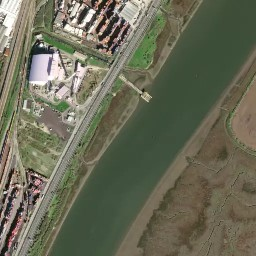
\includegraphics[width=\textwidth]{content/img/datensatz_satellite.jpg}
        \caption{Satellitenbild}
    \end{subfigure}
    \hfill
    \begin{subfigure}{0.48\textwidth}
        \centering
        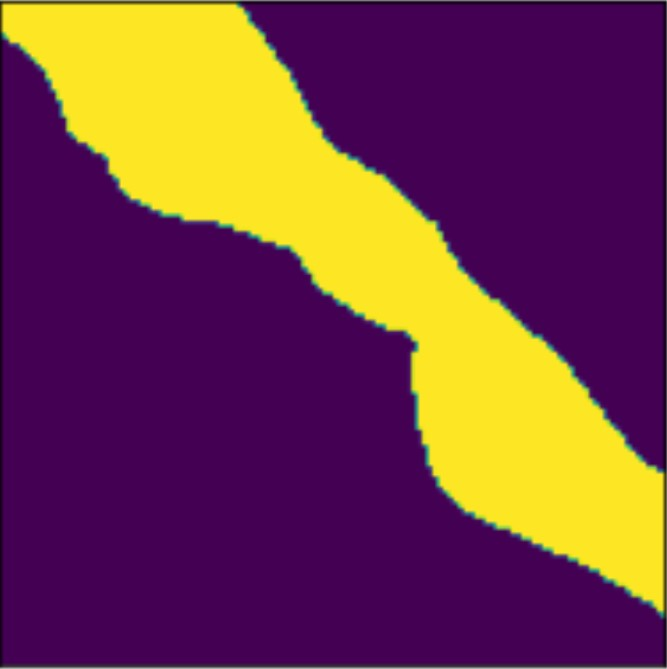
\includegraphics[width=\textwidth]{content/img/datensatz_mask.jpg}
        \caption{Maske}
    \end{subfigure}
    \caption{Beispiel aus dem Datensatz für ein Satellitenbild aus Littauen mit zugehöriger Maske.\cite{mapbox}}
    \label{fig:datensatz}
\end{figure}
\\
Der Datensatz wird mit Python über die API von Mapbox\cite{mapbox} generiert.
Europa hat einen Wasserflächenanteil von wenigen Prozent.
Um nun nicht größtenteils gewässerfreie Satellitenaufnahmen zu erhalten, muss geprüft werden ob sich in den gezogenen Koordinaten ein Fluss, See oder Meer befindet.
Die Vorgehensweise wird grob beschrieben:
\begin{itemize}
    \item generiere zufällige Koordinaten auf dem europäischen Festland (Ländergrenzen aus 'Natural Earth' \cite{naturalearth})
    \item prüfe ob Gewässer innerhalb eines 'Tiles'\footnote{\label{foot:tiles}Die Karte wird Abhängig von der Zoomstufe in unterschiedlich viele Quadrate unterteilt, sog. 'Tiles'.} vorkommen
    \item download des Satelliten- und Maskenbilds über Mapbox\cite{mapbox} \\
          per Link: \url{https://api.mapbox.com/v4/mapbox.satellite/{zoom}/{x}/{y}.mvt?access_token=\{token\}}
    \item skaliere Bilder von $256 \times 256$ zu $128 \times 128$
\end{itemize}